\documentclass[11pt]{article}

\usepackage[a4paper,margin=1in]{geometry}
\usepackage{amsmath}
\usepackage{graphicx}
\usepackage{listings}
\usepackage{xcolor}
\usepackage{booktabs}
\usepackage{tikz}
\usepackage{hyperref}
\usepackage{parskip}
\usetikzlibrary{arrows.meta,positioning}

\definecolor{codebg}{RGB}{245,245,245}
\definecolor{codekw}{RGB}{0,0,150}
\definecolor{codecomment}{RGB}{100,100,100}
\definecolor{codestring}{RGB}{150,0,0}

\lstdefinestyle{code}{
    backgroundcolor=\color{codebg},
    basicstyle=\ttfamily\footnotesize,
    keywordstyle=\color{codekw}\bfseries,
    commentstyle=\color{codecomment}\itshape,
    stringstyle=\color{codestring},
    numbers=left,
    numberstyle=\tiny\color{gray},
    numbersep=6pt,
    frame=single,
    breaklines=true,
    showstringspaces=false,
    tabsize=2,
    xleftmargin=1.5em,
}
\lstset{style=code}

\lstdefinelanguage{CFlex}{
    morekeywords={if,else,while,do,for,switch,case,default,break,continue,return,goto,int,char,float,double,void,long,short,unsigned,signed,const,static,struct},
    sensitive=true,
    morecomment=[l]{//},
    morecomment=[s]{/*}{*/},
    morestring=[b]"
}

\title{\textbf{Cyclomatic Complexity Analyzer for C Programs} \\
\large Design and Implementation of a Lexer--Parser--CFG Pipeline with Web-Based Visualization}
\author{Siddharth Narayan Mishra \\ Roll Number: 123CS0189}
\date{Software Testing Laboratory}

\begin{document}
\maketitle

\section{Aim}
To design and implement a tool that computes the \textbf{cyclomatic complexity} of functions written in the C programming language. The tool parses a C source file, builds a \textbf{Control Flow Graph (CFG)} for every function it contains, applies McCabe's cyclomatic complexity formula to each CFG, and presents the result through an interactive web interface that visualizes the graph alongside the source code.

\section{Theory}

\subsection{Cyclomatic Complexity}
Cyclomatic complexity, introduced by Thomas J. McCabe in 1976, is a static software metric used to measure the structural complexity of a program by counting the number of linearly independent paths through its control flow. It is widely used in software testing to:
\begin{itemize}
    \item Estimate the minimum number of test cases required to achieve branch coverage,
    \item Flag overly complex functions that are more likely to contain defects and are harder to maintain,
    \item Guide basis-path testing, where a set of independent paths through the CFG is chosen as the test suite.
\end{itemize}

For a control flow graph $G$ with a single entry and a single exit, McCabe's formula is
\begin{equation}
    M = E - N + 2P
\end{equation}
where
\begin{itemize}
    \item $E$ is the number of edges in the graph,
    \item $N$ is the number of nodes (basic blocks) in the graph,
    \item $P$ is the number of connected components (for a single function, $P = 1$).
\end{itemize}

Equivalently, $M$ can be computed as the number of decision points (predicate nodes such as \texttt{if}, \texttt{while}, \texttt{for}, \texttt{case}) plus one, since every binary decision adds exactly one edge more than it adds nodes.

\subsection{Control Flow Graphs}
A control flow graph represents a function as a directed graph in which:
\begin{itemize}
    \item Each node is a \textbf{basic block} — a maximal straight-line sequence of statements with no jumps into or out of its middle,
    \item Each edge represents a possible transfer of control between blocks,
    \item A single \textbf{ENTRY} node and a single \textbf{EXIT} node bound the function.
\end{itemize}
Branching constructs (\texttt{if}, loops, \texttt{switch}) split a block into a predicate node with two or more outgoing edges (labelled \texttt{true}/\texttt{false}, or \texttt{case} values), while sequential statements are merged into the same block wherever no jump target lies between them.

\section{Tools and Technologies}
\begin{table}[h]
\centering
\begin{tabular}{@{}ll@{}}
\toprule
\textbf{Component} & \textbf{Tool / Library} \\
\midrule
Lexical analysis & Flex (\texttt{lexer.l}) \\
Syntax analysis & GNU Bison (\texttt{parser.y}), LALR(1) grammar \\
AST \& CFG construction & C (\texttt{ast.c}, \texttt{cfg.c}), compiled with GCC \\
Macro/preprocessor handling & \texttt{gcc -E -P} (piped input) \\
Backend API & Node.js, Express, Multer (file upload) \\
Frontend UI & React (Vite), \texttt{@xyflow/react} (React Flow) \\
Graph auto-layout & \texttt{dagre.js} \\
\bottomrule
\end{tabular}
\caption{Tools used across the pipeline}
\end{table}

\section{System Architecture}
The system is organized as three independently runnable components that communicate over HTTP, and internally the analyzer itself is a compiler-style pipeline. Figure~\ref{fig:pipeline} shows the overall flow from a \texttt{.c} source file to the rendered CFG in the browser.

\begin{figure}[h]
\centering
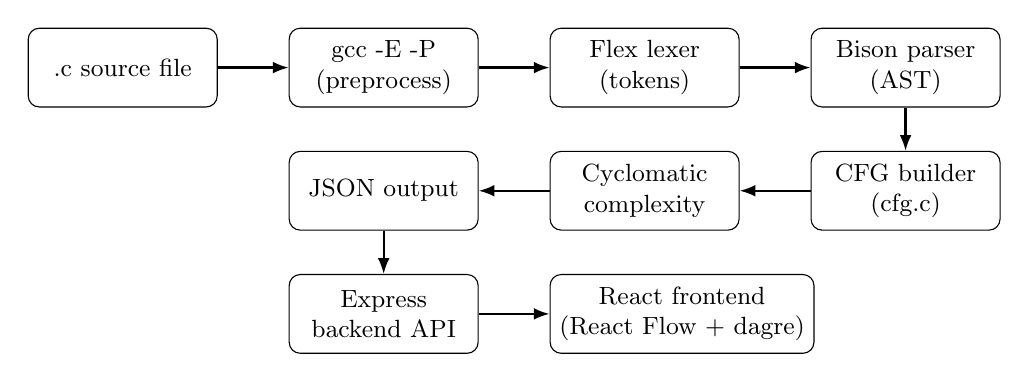
\begin{tikzpicture}[
    node distance=0.55cm and 0.9cm,
    box/.style={draw, rounded corners, minimum height=1cm, minimum width=2.4cm, align=center, font=\small},
    arr/.style={-{Latex[length=2mm]}, thick}
]
\node[box] (src) {.c source file};
\node[box, right=of src] (pp) {gcc -E -P\\(preprocess)};
\node[box, right=of pp] (lex) {Flex lexer\\(tokens)};
\node[box, right=of lex] (par) {Bison parser\\(AST)};
\node[box, below=of par] (cfg) {CFG builder\\(cfg.c)};
\node[box, left=of cfg] (mccabe) {Cyclomatic\\complexity};
\node[box, left=of mccabe] (json) {JSON output};
\node[box, below=of json] (api) {Express\\backend API};
\node[box, right=of api] (react) {React frontend\\(React Flow + dagre)};

\draw[arr] (src) -- (pp);
\draw[arr] (pp) -- (lex);
\draw[arr] (lex) -- (par);
\draw[arr] (par) -- (cfg);
\draw[arr] (cfg) -- (mccabe);
\draw[arr] (mccabe) -- (json);
\draw[arr] (json) -- (api);
\draw[arr] (api) -- (react);
\end{tikzpicture}
\caption{End-to-end pipeline: source $\rightarrow$ preprocessing $\rightarrow$ lexing $\rightarrow$ parsing $\rightarrow$ AST $\rightarrow$ CFG $\rightarrow$ complexity $\rightarrow$ JSON $\rightarrow$ backend API $\rightarrow$ frontend visualization.}
\label{fig:pipeline}
\end{figure}

\begin{enumerate}
    \item \textbf{Parser (C, \texttt{parser/})}: a native binary, \texttt{cflow-analyzer}, built from a Flex lexer and a Bison grammar. It reads one \texttt{.c} file, builds an abstract syntax tree (AST), constructs one CFG per function, computes the cyclomatic complexity of each, and emits a JSON document describing every basic block and edge.
    \item \textbf{Backend (Node.js/Express, \texttt{backend/})}: a thin HTTP wrapper that invokes the compiled binary as a subprocess (\texttt{execFile}) on an uploaded or sample \texttt{.c} file and streams its JSON output back to the browser.
    \item \textbf{Frontend (React, \texttt{frontend/})}: renders the CFG returned by the backend as an interactive node-link diagram, shows the source file with click-to-locate highlighting between source lines and CFG nodes, and displays the $M = E - N + 2P$ computation for the selected function.
\end{enumerate}

\section{Implementation}

\subsection{Lexical Analysis}
The lexer (\texttt{lexer.l}) tokenizes a preprocessed C source file. Since macro expansion and conditional compilation (\texttt{\#ifdef}) are already resolved by \texttt{gcc -E} before the lexer ever sees the input, the lexer itself only needs to recognize:
\begin{itemize}
    \item C keywords (\texttt{if}, \texttt{else}, \texttt{while}, \texttt{for}, \texttt{switch}, \texttt{case}, \texttt{return}, type keywords, etc.),
    \item identifiers, integer/float/hex/character constants, and string literals,
    \item multi-character operators (\texttt{++}, \texttt{->}, \texttt{<=}, \texttt{\&\&}, compound assignment operators, \ldots),
    \item single-character punctuation, forwarded verbatim as their own token.
\end{itemize}
Comments and residual \texttt{gcc -E} linemarker lines (e.g.\ \texttt{\# 1 "file.c"}) are discarded in the lexer itself.

\subsection{Syntax Analysis and AST Construction}
\begin{sloppypar}
The grammar (\texttt{parser.y}) is a Bison LALR(1) grammar implementing a practical subset of C89-style expression and statement syntax: function definitions, all standard statement forms (\texttt{if}/\texttt{else}, \texttt{while}, \texttt{do\ldots while}, \texttt{for}, \texttt{switch}/\texttt{case}/\texttt{default}, \texttt{break}, \texttt{continue}, \texttt{return}, \texttt{goto}/labels), declarations, and the full C expression-precedence chain. The precedence chain runs from \texttt{primary\_expr} up through \texttt{assignment\_expr}, and uses the classic \texttt{\%prec LOWER\_THAN\_ELSE} technique to resolve the dangling-else ambiguity.
\end{sloppypar}

Rather than building a full C type system, each expression rule reconstructs and returns its own source text (e.g. \texttt{"a[i] < 0"}) which is later used verbatim as the label of the basic block it is attached to. Each statement is represented as an \texttt{Stmt} node (Listing~\ref{lst:asth}) tagged with a \texttt{StmtType} and up to four child-statement pointers, whose meaning depends on the type of statement (e.g.\ \texttt{s1}/\texttt{s2} are the then/else branches of an \texttt{if}, while \texttt{s1} is the loop body of a \texttt{while}).

\begin{lstlisting}[language=C, caption={Core AST node definition (\texttt{ast.h})}, label={lst:asth}]
typedef enum {
    STMT_COMPOUND, STMT_IF, STMT_WHILE, STMT_DO_WHILE, STMT_FOR,
    STMT_SWITCH, STMT_CASE, STMT_DEFAULT, STMT_BREAK, STMT_CONTINUE,
    STMT_RETURN, STMT_GOTO, STMT_LABEL, STMT_EXPR, STMT_DECL, STMT_EMPTY
} StmtType;

typedef struct Stmt {
    StmtType type;
    int line;
    char *text;                     /* expr / cond / label / goto target */
    char *text2, *text3;            /* STMT_FOR only: init, incr */
    struct Stmt *s1, *s2, *s3, *s4; /* meaning depends on type */
    struct StmtList *body;          /* STMT_COMPOUND: statements in block */
} Stmt;
\end{lstlisting}

\subsection{Control Flow Graph Construction}
The CFG builder (\texttt{cfg.c}) walks the AST of each function once, threading a ``current block'' pointer through the statement list and emitting new basic blocks and edges as control-flow constructs are encountered. Table~\ref{tab:cfgrules} summarizes the graph fragment generated for each construct.

\begin{table}[h]
\centering
\small
\begin{tabular}{@{}p{2.6cm}p{9.6cm}@{}}
\toprule
\textbf{Construct} & \textbf{CFG fragment emitted} \\
\midrule
Sequential statement & Appended as another line into the current block; no new node. \\
\texttt{if}/\texttt{else} & Condition ends the current block; \texttt{true} edge to a new then-block, \texttt{false} edge to a new else-block (or directly to the join block if no \texttt{else}); both branches merge into a new join block. \\
\texttt{while} & New header block holding the condition; \texttt{true} edge into the body, \texttt{false} edge to the exit block; the body's fall-through edges back to the header. \\
\texttt{do\ldots while} & Body executes unconditionally once; the trailing condition block has a \texttt{true} edge back to the body and a \texttt{false} edge to the exit. \\
\texttt{for} & Init text is appended to the entry block; a header block holds the condition (\texttt{true}$\to$body, \texttt{false}$\to$exit); the body's exit unconditionally reaches an increment block, which loops back to the header. \\
\texttt{switch} & Each \texttt{case}/\texttt{default} becomes its own block reached by a \texttt{case}-labelled edge from the switch's condition block; blocks without a preceding \texttt{break} fall through to the next case block, matching real C semantics. \\
\texttt{break} / \texttt{continue} & Unconditional edge to the innermost enclosing loop's exit block / loop-continuation block, tracked via explicit stacks (\texttt{break\_stack}, \texttt{continue\_stack}). \\
\texttt{return} & Unconditional edge straight to the function's single \texttt{EXIT} node. \\
\texttt{goto}/label & Recorded as a pending jump and resolved in a second pass once every label in the function has been visited, since a \texttt{goto} may jump forward. \\
\bottomrule
\end{tabular}
\caption{Mapping from AST statement types to CFG fragments}
\label{tab:cfgrules}
\end{table}

Every function's CFG has exactly one \texttt{ENTRY} block and one \texttt{EXIT} block, so $P = 1$ always holds, which is what allows the simplified formula $M = E - N + 2$ to be used directly (Listing~\ref{lst:mccabe}).

\begin{lstlisting}[language=C, caption={Cyclomatic complexity computation (\texttt{cfg.c})}, label={lst:mccabe}]
int cyclomatic_complexity(CFG *cfg) {
    /* M = E - N + 2P, P = 1 (single entry/exit per function) */
    return cfg->num_edges - cfg->num_blocks + 2;
}
\end{lstlisting}

Once every CFG is built, \texttt{cfg\_to\_json()} serializes each function's node list (id, source-line range, label text) and edge list (source, target, edge type, optional case label) to a JSON document that is written to stdout or a given output file.

\subsection{Backend and Frontend}
The Express backend (\texttt{server.js}) exposes two endpoints: \texttt{GET /api/sample}, which analyzes a bundled example file, and \texttt{POST /api/analyze}, which accepts an uploaded \texttt{.c} file (via Multer, capped at 1\,MB), writes it to a temporary path, and invokes the compiled analyzer binary as a subprocess before returning its JSON output. Both endpoints respond with the original source text alongside the per-function CFG data so the frontend can correlate graph nodes with source lines.

The React frontend renders the selected function's CFG using \texttt{@xyflow/react}, with node positions computed automatically by \texttt{dagre}'s layered (Sugiyama-style) layout algorithm. Edges are colour-coded by type (true/false/unconditional/case), and clicking a node highlights the corresponding source-line range, while clicking a source line highlights the block that contains it. A metrics panel displays $N$, $E$, $P$, and the resulting $M$ for the active function.

\section{Results}
The analyzer was run on two hand-written test programs, \texttt{sample1.c} and \texttt{sample2.c}, exercising \texttt{if}/\texttt{else if} chains, loops (\texttt{while}, \texttt{do\ldots while}, \texttt{for}, nested \texttt{for}), \texttt{switch} with fall-through, and a \texttt{goto}. Table~\ref{tab:results} shows the computed metrics for every function.

\begin{table}[h]
\centering
\begin{tabular}{@{}llccc@{}}
\toprule
\textbf{File} & \textbf{Function} & \textbf{Nodes ($N$)} & \textbf{Edges ($E$)} & \textbf{Complexity ($M$)} \\
\midrule
sample1.c & \texttt{classify}           & 8  & 9  & 3 \\
sample1.c & \texttt{sumEvens}           & 8  & 9  & 3 \\
sample1.c & \texttt{gradeOf}            & 8  & 11 & 5 \\
sample1.c & \texttt{findFirstNegative}  & 7  & 8  & 3 \\
\midrule
sample2.c & \texttt{binarySearch}       & 11 & 13 & 4 \\
sample2.c & \texttt{validateAndSum}     & 12 & 14 & 4 \\
sample2.c & \texttt{collatzSteps}       & 8  & 9  & 3 \\
sample2.c & \texttt{categorize}         & 10 & 15 & 7 \\
sample2.c & \texttt{gcd}                & 5  & 5  & 2 \\
sample2.c & \texttt{matrixTrace}        & 12 & 14 & 4 \\
\bottomrule
\end{tabular}
\caption{Cyclomatic complexity of every function in the two test programs}
\label{tab:results}
\end{table}

These results match hand-verified expectations: \texttt{gcd} has a single loop and no other branching, giving $M=2$ (one decision point plus one); \texttt{categorize} has the highest complexity because its six-way \texttt{switch} contributes one decision edge per \texttt{case} label.

\subsection{Worked Example: \texttt{classify()}}
Consider the following function from \texttt{sample1.c}:
\begin{lstlisting}[language=C]
int classify(int x) {
    int result = 0;
    if (x < 0) {
        result = -1;
    } else if (x == 0) {
        result = 0;
    } else {
        result = 1;
    }
    return result;
}
\end{lstlisting}
The tool decomposes this into 8 basic blocks and 9 edges (Figure~\ref{fig:classify}): an entry block holding the declaration and the first condition, two nested decision blocks (from the \texttt{if}/\texttt{else if} chain), three assignment blocks, a join block, and the return/exit blocks.

\begin{figure}[h]
\centering
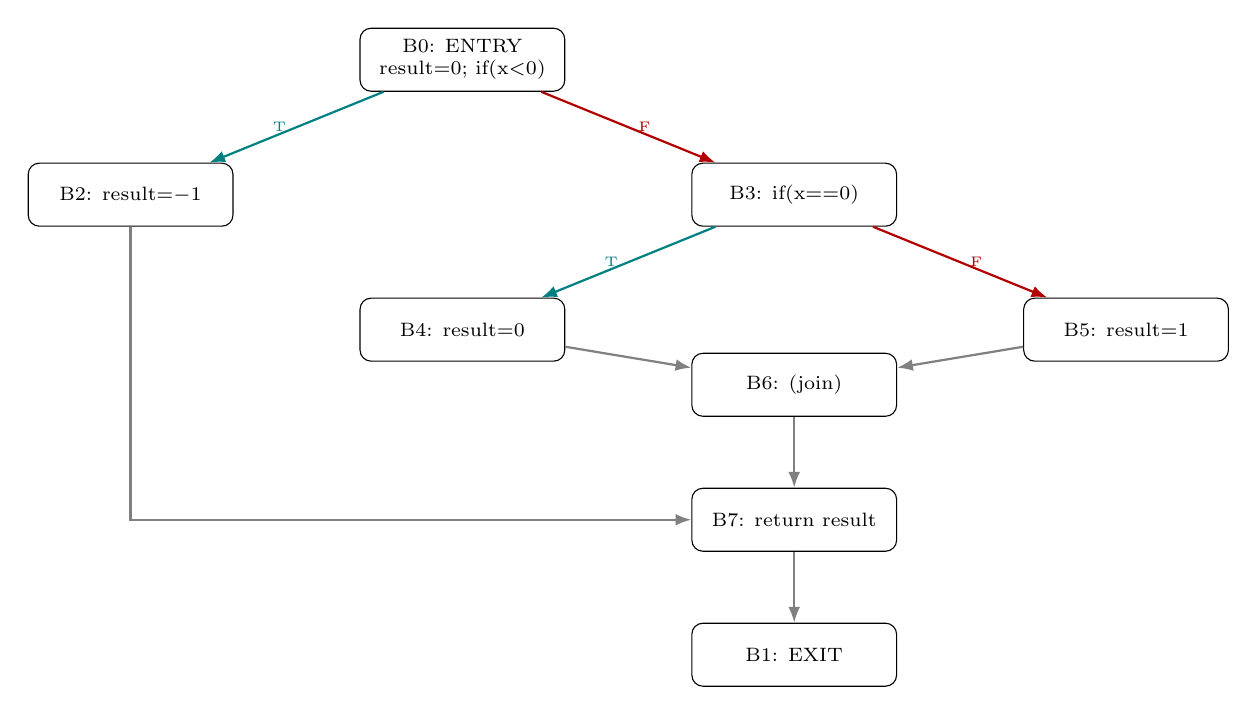
\begin{tikzpicture}[
    node distance=0.9cm and 1.6cm,
    blk/.style={draw, rounded corners, minimum width=2.6cm, minimum height=0.8cm, align=center, font=\scriptsize},
    arr/.style={-{Latex[length=2mm]}, thick},
    t/.style={arr, teal},
    f/.style={arr, red!70!black},
    u/.style={arr, gray}
]
\node[blk] (b0) {B0: ENTRY\\result=0; if(x$<$0)};
\node[blk, below left=of b0] (b2) {B2: result=$-1$};
\node[blk, below right=of b0] (b3) {B3: if(x==0)};
\node[blk, below left=of b3] (b4) {B4: result=0};
\node[blk, below right=of b3] (b5) {B5: result=1};
\node[blk, below=1.6cm of b3] (b6) {B6: (join)};
\node[blk, below=of b6] (b7) {B7: return result};
\node[blk, below=of b7] (b1) {B1: EXIT};

\draw[t] (b0) -- node[left,font=\tiny]{T} (b2);
\draw[f] (b0) -- node[right,font=\tiny]{F} (b3);
\draw[t] (b3) -- node[left,font=\tiny]{T} (b4);
\draw[f] (b3) -- node[right,font=\tiny]{F} (b5);
\draw[u] (b4) -- (b6);
\draw[u] (b5) -- (b6);
\draw[u] (b2) |- (b7);
\draw[u] (b6) -- (b7);
\draw[u] (b7) -- (b1);
\end{tikzpicture}
\caption{CFG generated for \texttt{classify()}: $N=8$, $E=9$, so $M = 9 - 8 + 2 = 3$.}
\label{fig:classify}
\end{figure}

Applying the formula: $M = E - N + 2P = 9 - 8 + 2(1) = 3$, matching the two \texttt{if} decision points plus one, and agreeing exactly with the tool's own output. This also indicates that three independent test cases -- $x<0$, $x=0$, and $x>0$ -- are sufficient to exercise every branch of the function, which is precisely the practical use of cyclomatic complexity in basis-path testing.

\section{Known Limitations}
The current implementation targets a practical subset of C sufficient for algorithmic function bodies, and does not attempt full ISO C conformance:
\begin{itemize}
    \item No \texttt{typedef} support, and consequently no ``lexer hack'' to disambiguate typedef'd type names from identifiers.
    \item No explicit type-cast expressions, e.g.\ \texttt{(int)x}.
    \item \texttt{\#include}d headers are stripped before parsing rather than resolved -- only the function bodies defined in the user's own file are analyzed.
    \item Global variable declarations support only a single declarator per line.
\end{itemize}

\section{Conclusion}
This lab exercise implements a complete, working front-to-back pipeline for static analysis of C programs: a Flex/Bison compiler front end builds an AST from C source, a graph-construction pass turns each function's AST into a control flow graph following well-defined per-construct rules, and McCabe's cyclomatic complexity formula $M = E - N + 2P$ is applied directly to the resulting graph. Wrapping the analyzer in an HTTP API and a React-based visualizer made it possible to inspect and verify the generated CFGs interactively, which was invaluable for validating tricky constructs such as \texttt{switch} fall-through and forward \texttt{goto} resolution against their expected complexity values. The exercise reinforced both the theory of control-flow-based test-adequacy criteria and the practical mechanics of building a small compiler front end with Flex and Bison.

\end{document}
